\section{Metodo delle tangenti}
Fino ad ora abbiamo scelto come funzione $g$ per il metodo iterativo qualcosa nella forma
\[ g(x) = x - f(x) \]
Per il metodo che vedremo tra poco scegliamo invece $g$ nella forma
\[ g(x) = x - \frac{f(x)}{g(x)} \]
Dove $h(x)$ ricordiamo essere una funzione definita sugli \emph{zeri} di $f$. Il metodo che vediamo è chiamato
\textbf{metodo delle tangenti} o \textbf{metodo di Newton} e prende $h(x) = f'(x)$ definendo $g(x)$ come segue
\[ g(x) = x - \frac{f(x)}{f'(x)} \]
Otteniamo quindi il seguente metodo iterativo
\[ x_{k+1} = x_k - \frac{f(x_k)}{f'(x_k)} \]
Supponiamo di avere una funzione $f$ e di voler trovare $\alpha$ tale che $f(\alpha) = 0$. Supponiamo ora di
avere un punto $x_0$ e il valore della funzione calcolata in tale punto, ossia $f(x_0)$. Otteniamo così il
punto $(x_0, f(x_0)) \in f$.

Definiamo ora la retta tangente alla funzione passante per tale punto. L'equazione della tangente alla funzione
è la seguente
\[ y - f(x_0) = f'(x_0)(x - x_0) \]
Andiamo ora a calcolare l'intersezione della tangente con l'asse delle ascisse trovando così il nuovo punto $x_1$.
\[
	\begin{cases}
		y - f(x_0) = f'(x_0)(x_1 - x_0) \\
		y = 0
	\end{cases}
\]
Sostituendo $y = 0$ nella prima equazione otteniamo
\begin{align*}
	-f(x_0) =                 & f'(x_0)(x_1 - x_0)           \\
	-\frac{f(x_0)}{f'(x_0)} = & x_1 - x_0                    \\
	x_1 =                     & x_0 - \frac{f(x_0)}{f'(x_0)}
\end{align*}
Ecco che abbiamo ottenuto l'equazione di partenza del metodo. A questo punto non ci rimane che ripetere il
procedimento per $x_1$ fino a quando il metodo non converge.

La derivata di $g(x) = x - \frac{f(x)}{f'(x)}$, in questo caso, è la seguente
\[ g'(x) = 1 - \frac{f'(x) f'(x) - f''(x) f(x)}{f'(x)^2} = \frac{f''(x) f(x)}{f'(x)^2} \]
Se valutiamo $g'$ in $\alpha$ otteniamo
\[ g'(\alpha) = \frac{f''(\alpha) f(\alpha)}{f'(\alpha)^2} \]
Teniamo a mente però che $\alpha$ è radice della funzione $f$ e quindi vale
\[ f(\alpha) = 0 \quad \Rightarrow \quad g'(\alpha) = 0 < 1 \]
se $f'(\alpha) \neq 0$.Dunque, sotto quest'ipotesi, il metodo converge localmente.

\begin{example}
	Proviamo ora a calcolare la radice $\alpha$ dell'equazione
	\[ f(x) = e^{-x} - x = 0 \]
	con il metodo delle tangenti. Calcoliamo la derivata prima
	\[ f'(x) = -e^{-x} - 1 \]
	Supponiamo di scegliere $x_0 = 0$ e valutiamo la funzione in $x_0$, ottenendo il punto $(0, 1)$ da cui
	iniziare a iterare. La tangente $t_0$ alla funzione nel punto trovato ha equazione
	\[ y = -2x + 1 \]
	Calcoliamo quindi il punto $x_1$ ponendo $y=0$ e otteniamo $x_1 = \frac{1}{2}$
	Se adesso ripetiamo il procedimento otteniamo la tangente $t_1$ della funzione nel punto
	$(x_1, f(x_1)) = \left( \frac{1}{2}, \frac{1}{\sqrt{e}} - \frac{1}{2} \right)$, ossia
	\[ y = - x \left( \frac{1}{\sqrt{e}} + 1 \right) + \frac{3}{2 \sqrt{e}} \]
	\begin{center}
		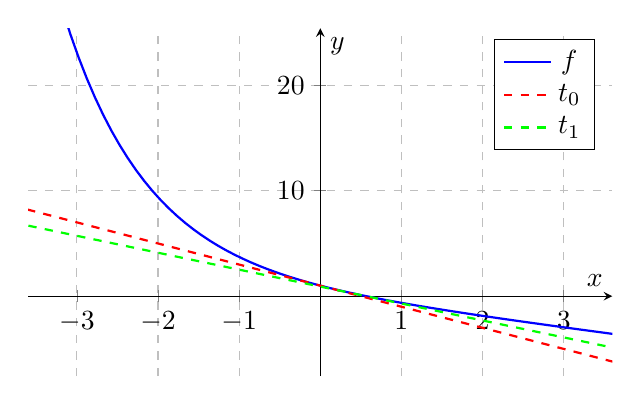
\begin{tikzpicture}
			\begin{axis}[
					font=\normalsize,
					width=9cm,
					height=6cm,
					axis lines = center,
					xlabel = $x$,
					ylabel = $y$,
					xmin = -3, xmax = 3,
					grid = both,
					grid style = dashed,
					legend pos = north east,
					enlargelimits
				]

				\addplot [ samples=100, thick, color=blue ] {exp(-x) - x};

				\addplot [ thick, dashed, color=red] {-2 * x + 1};

				\addplot [thick, dashed, color=green] { - 1.606 * x + 0.909 };

				\legend{ $f$, $t_0$, $t_1$ }
			\end{axis}
		\end{tikzpicture}
	\end{center}
	Come possiamo vedere, la seconda tangente (in verde) incontra l'asse delle ascisse in un punto più vicino ad
	$\alpha$.
\end{example}

Nel caso in cui $f'(\alpha) = 0$ il metodo converge comunque anche se non possiamo dire di avere convergenza
locale.

\begin{example}
	Consideriamo ora l'equazione
	\[ f(x) = x^2 = 0 \]
	Vediamo facilmente che l'equazione ha due radici reali coincidenti $\alpha = \beta = 0$. La derivata prima
	equivale però a
	\[ f'(x) = 2x \]
	e quindi $f'(0) = 0$. Andiamo però ad analizzare la successione generata dal metodo delle tangenti.
	\[ x_{k+1} = x_k - \frac{x_k^2}{2 x_k} = x_k - \frac{x_k}{2} = \frac{x_k}{2} \]
	Ogni elemento della successione è la metà del precedente e quindi l'elemento al passo $(k+1)$-esimo equivale a
	\[ x_{k+1} = \frac{x_0}{2^k} \]
	Ed è facile notare che
	\[ \lim_{k \to +\infty} \frac{x_0}{2^k} = 0 \]
	qualsiasi sia $x_0$, dunque il metodo è convergente.
\end{example}